\documentclass[12pt]{article}

\usepackage{sbc-template}

\usepackage{graphicx,url}
\usepackage[utf8]{inputenc}
\usepackage[brazil]{babel}
\usepackage{amsmath}
\usepackage{booktabs}
\usepackage{hyperref}

\sloppy

\title{Previsão de Picos de Crimes Violentos e de Sinistros de Trânsito em
Dias de Jogos de Futebol na Cidade de São Paulo}

\author{Gilberto Serafim Dias de Araújo\inst{1}, Leonardo de Cico\inst{1},
Pedro Henrique de Almeida\inst{1}}

\address{Universidade de São Paulo (USP)\\
  São Paulo -- SP -- Brasil
  \email{serafimgilberto0@usp.br, leocico@usp.br, pedroalmeida04@usp.br}
}

\begin{document}

\maketitle

\begin{resumo}
Partidas de futebol concentram multidões em torno de estádios e alteram, por
algumas horas, as rotinas de deslocamento e convívio de uma cidade inteira.
Este trabalho construiu uma tabela analítica diária (730 dias, 2022--2023)
integrando o calendário de partidas dos clubes de São Paulo capital,
registros oficiais de criminalidade e de sinistros de trânsito, e variáveis
de clima e calendário, e investigou empiricamente se dias de jogo se
associam a picos desses desfechos e se essa associação é preditiva e/ou
causal. Sete abordagens metodológicas independentes -- comparação ajustada
por GLM Poisson, correlação parcial, modelo de defasagens distribuídas,
\emph{Difference-in-Differences} espacial, \emph{Propensity Score Matching}
com IPTW, uma adaptação de \emph{Interrupted Time Series} e auditoria de
colinearidade em valores de SHAP -- convergem em um mesmo resultado: a
associação bruta observada desaparece após controle por calendário, e
nenhum método encontra evidência causal robusta de efeito do futebol. Um
modelo XGBoost com função de perda de Poisson superou os \emph{baselines}
e o Prophet na previsão da contagem diária de crimes violentos (MAE~34,8) e
de sinistros com vítima (MAE~10,3), validado por janela expansiva
\emph{walk-forward}; uma Regressão Logística balanceada atingiu Recall de
0,58 na identificação de dias de pico de sinistros com vítima, mas nenhum
classificador testado chegou a um ponto de operação útil para crimes
violentos. Os resultados indicam que sistemas de alerta operacional para
esses desfechos em São Paulo devem se apoiar em padrão histórico do próprio
desfecho, calendário civil e clima -- não no calendário de jogos de
futebol.
\end{resumo}

\begin{abstract}
Football matches concentrate crowds around stadiums and disrupt, for a few
hours, the commuting and social routines of an entire city. This work built
a daily analytical table (730 days, 2022--2023) integrating the match
calendar of São Paulo football clubs, official records of criminal
occurrences and traffic accidents, and weather and calendar variables, and
empirically investigated whether game days are associated with peaks in
these outcomes, and whether that association is predictive and/or causal.
Seven independent methodological approaches -- adjusted Poisson GLM
comparison, partial correlation, distributed-lag model, spatial
Difference-in-Differences, Propensity Score Matching with IPTW, an adapted
Interrupted Time Series, and a SHAP collinearity audit -- converge on the
same result: the raw association disappears after controlling for
calendar, and no method finds robust causal evidence of a football effect.
An XGBoost model with a Poisson loss outperformed baselines and Prophet in
forecasting daily counts of violent crime (MAE~34.8) and injury traffic
accidents (MAE~10.3), validated by expanding-window walk-forward
validation; a balanced Logistic Regression reached a Recall of 0.58 for
identifying injury-accident peak days, but no classifier tested reached a
useful operating point for violent crime. The results indicate that
operational alert systems for these outcomes in São Paulo should rely on
the outcome's own historical pattern, civil calendar and weather -- not on
the football match schedule.
\end{abstract}

\section{Introdução}

Grandes eventos esportivos são, do ponto de vista urbano, deslocamentos
temporários de rotina. Em poucas horas, dezenas de milhares de pessoas se
concentram no entorno de um estádio, alteram trajetos habituais, consomem
álcool em bares e praças de concentração e retornam simultaneamente para
casa ao final da partida. A Teoria da Atividade Rotineira \cite{cohen1979}
descreve exatamente esse cenário como propício à ocorrência de crimes: a
convergência, no tempo e no espaço, de ofensores motivados, alvos
disponíveis e ausência de vigilância capaz. São Paulo é um caso extremo
desse fenômeno no Brasil, por concentrar três clubes de série A que mandam
jogos na capital, quatro estádios de grande porte e uma agenda que, entre
campeonatos estadual, nacional, copas e competições continentais, raramente
deixa uma semana sem jogo na cidade. Ao mesmo tempo, a disponibilidade de
dados abertos sobre segurança pública, sinistros de trânsito e clima tornou
tecnicamente viável investigar essa relação com métodos quantitativos, o
que até pouco tempo dependia de coleta manual.

O problema tratado neste trabalho é a investigação, em nível diário e para
o município de São Paulo, da associação entre partidas de futebol e dias
atípicos de violência e de sinistros de trânsito, e da possibilidade de
antecipar esses dias a partir do calendário de jogos, das características
de cada partida (mandante, horário, clássico), do clima e do calendário
civil. A pergunta que orientou a investigação é concreta: conhecendo essas
variáveis com antecedência de um dia, é possível estimar se determinada
data terá volume de ocorrências acima do padrão -- e, indo além da
predição, existe evidência de que o jogo em si, e não o calendário que o
circunda, é responsável por essa eventual elevação? A unidade de análise é
o dia na cidade -- não se pretendeu localizar espacialmente cada
ocorrência -- e o produto é uma estimativa de risco potencialmente
utilizável no planejamento de efetivo policial e de fiscalização de
trânsito.

Três dificuldades motivaram esta investigação. A primeira é metodológica:
os trabalhos de referência \cite{kurland2014,ristea2018,ristea2020} são
espaciais e explicativos, em escala muito mais fina do que a cidade
inteira. A segunda é de disponibilidade de dados: parte do ganho preditivo
relatado nesses estudos vem de mensagens geolocalizadas de redes sociais,
fonte cujo acesso programático foi drasticamente restringido, tornando
necessário verificar quanto sinal permanece recuperável apenas com dados
oficiais e de calendário. A terceira é a escassez de estudos que tratem
crimes e sinistros de trânsito como alvos de um mesmo pipeline, apesar de
compartilharem determinantes semelhantes em dias de jogo -- aglomeração,
álcool, deslocamento noturno concentrado.

O objetivo geral foi construir e avaliar um sistema de ciência de dados
que investigasse essa associação e estimasse o risco em granularidade
diária, com quatro objetivos específicos: (i) levantar e integrar as
fontes públicas necessárias; (ii) especificar um pipeline que consolidasse
fontes de granularidades distintas numa tabela analítica diária única;
(iii) formular a tarefa preditiva e um critério não arbitrário de pico,
validado temporalmente; e (iv) ir além da predição, aplicando métodos de
inferência causal observacional para verificar se a associação resiste ao
controle por confundidores de calendário -- objetivo que extrapolou a
ambição inicial do projeto e se tornou um dos resultados centrais deste
trabalho.

\section{Trabalhos Relacionados}

Kurland et al. \cite{kurland2014} examinaram o entorno do Villa Park
(Birmingham) e mostraram que a distribuição espacial de furtos e crimes
violentos difere significativamente entre dias de jogo e dias de controle
num raio de $\sim$3\,km do estádio -- estabelecendo o desenho de dias de
evento contra controle e evidenciando que o efeito, quando existe, não se
restringe ao perímetro imediato do estádio, o que motivou aqui testar
tanto a escala de bairro quanto a cidade inteira.

Ristea et al. \cite{ristea2018} combinaram dados criminais
georreferenciados com mensagens do Twitter em células de
500\,m$\times$500\,m ao redor de um estádio, mostrando que mensagens de
conteúdo violento correlacionam-se espacialmente mais com crime do que o
volume total de mensagens -- achado que sustenta um princípio adotado
aqui: subconjuntos qualificados de um evento (clássicos, jogos noturnos)
podem ser mais informativos que o agregado indiferenciado. Em trabalho
posterior, Ristea et al. \cite{ristea2020} estenderam a abordagem para
Chicago com modelos de previsão espacial para sete tipos de crime; a
inclusão de redes sociais elevou a AUC de forma heterogênea entre
categorias, motivando aqui também uma leitura desagregada por grupo de
atributos.

Os três trabalhos convergem em limitações que condicionam esta
investigação: defasagem e granularidade heterogênea entre bases, e o
problema da unidade de área modificável (MAUP). O posicionamento deste
trabalho é triplo: deslocou-se do objetivo espacial de fina granularidade
para um objetivo temporal agregado à cidade inteira; substituiu-se a fonte
dinâmica de redes sociais -- indisponível em escala para o caso brasileiro
-- por atributos de partida conhecidos com antecedência, tratando
conjuntamente crimes e sinistros como alvos do mesmo pipeline; e,
diferentemente dos trabalhos de referência (objetivo primariamente
explicativo-espacial), formalizou-se um bloco de inferência causal
observacional (pareamento por escore de propensão, IPTW, adaptação de
séries temporais interrompidas) que explicita o quanto a associação
resiste ao controle por confundidores.

% =====================================================================
% SEÇÃO 3 — METODOLOGIA
% Estrutura inspirada em:
%   - da Silva, Rodrigues-Jr & de Albuquerque (2025), "On the power of CNNs
%     to detect slums in Brazil", Computers, Environment and Urban Systems
%     (estágios numerados: aquisição -> processamento -> treino -> análise)
%   - Soliani et al. (2024), "Catastrophic causes of truck drivers' crashes
%     on Brazilian highways", Multimodal Transportation
%     (bloco explicativo/causal primeiro, bloco preditivo depois)
% =====================================================================

\section{Metodologia}

A metodologia está organizada em dois blocos, seguindo a lógica adotada
por Soliani et al. \cite{soliani2024} ao investigar acidentes com
caminhões em rodovias brasileiras: um bloco explicativo, que estabelece se
e como o calendário de jogos se associa aos desfechos de interesse, e um
bloco preditivo, que usa essa base para construir e validar modelos de
previsão de picos. A Figura~\ref{fig:pipeline} resume as quatro etapas do
pipeline -- integração de dados, análise exploratória e causal, definição
do alvo e engenharia de atributos, e modelagem preditiva --, no espírito
do diagrama de estágios de da Silva et al. \cite{dasilva2025}.

\begin{figure}[ht]
\centering
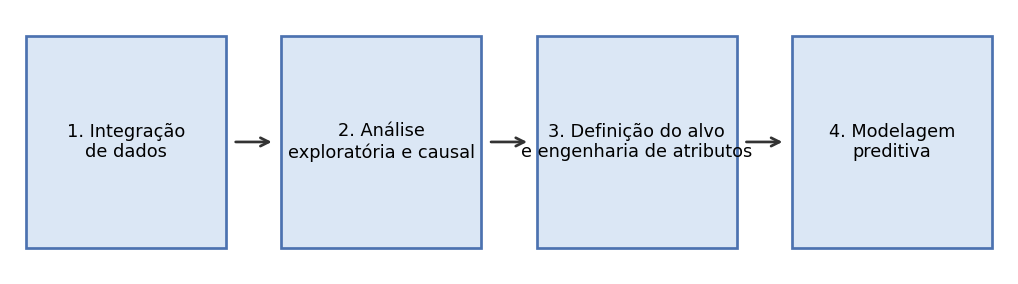
\includegraphics[width=.95\linewidth]{figuras/pipeline.png}
\caption{Etapas do pipeline de dados e análise}
\label{fig:pipeline}
\end{figure}

\subsection{Fontes de dados e integração}

Quatro categorias de dados públicos foram integradas para o município de
São Paulo, no período de 2022-01-01 a 2023-12-31 (730 dias, a janela de
sobreposição entre as três fontes principais):

\begin{itemize}
\item \textbf{Criminalidade} -- SPDadosCriminais (SSP-SP), microdados de
  boletim de ocorrência (grão real é BO$\times$rubrica, não BO único),
  filtrados por código IBGE do município (3550308, mais confiável que o
  campo textual da cidade, que tem variantes de grafia/espaço em branco);
\item \textbf{Sinistros de trânsito} -- Infosiga SP (Detran-SP), mesmo
  filtro geográfico, granularidade de evento, \emph{encoding} latin-1;
\item \textbf{Partidas de futebol} -- base histórica do Campeonato
  Brasileiro (Séries A/B/C) e Copa do Brasil (2014--2023), restrita aos
  mandantes que jogam na capital (Corinthians, Palmeiras e São Paulo FC --
  o Santos manda em Santos-SP, fora do escopo como mandante); clássico
  definido como mandante \emph{e} visitante pertencentes a
  \{Corinthians, Palmeiras, São Paulo, Santos\};
\item \textbf{Clima e calendário} -- estação INMET A701 (Mirante),
  agregada de horária (UTC) para diária (Brasília, $-3$h fixo, sem
  horário de verão), mais feriados (calculados por algoritmo de Páscoa,
  sem depender de API externa) e calendário escolar da rede municipal
  (transcrito manualmente de resoluções oficiais).
\end{itemize}

Cada fonte foi agregada ao grão \emph{dia} e unida por uma chave de
calendário mestre, garantindo que dias sem jogo, chuva ou ocorrência
apareçam com valor zero explícito, não como linha ausente. Dois cuidados
de qualidade afetam diretamente a validade das análises subsequentes:
os últimos dois dias da série (30--31/12/2023) têm contagens anormalmente
baixas por defasagem no registro administrativo, não queda real, e foram
excluídos de todos os testes e treinamentos; e um dia isolado
(19/06/2022) tem um pico de furtos compatível com lançamento retroativo em
lote, cujo tratamento foi avaliado por análise de sensibilidade.

\subsection{Bloco explicativo: associação entre jogos e desfechos}

Antes de qualquer modelo preditivo, testou-se se dias de jogo se associam
a desfechos elevados de criminalidade e sinistros, e se essa associação
sobrevive ao controle por calendário -- réplica do cuidado de Soliani et
al. \cite{soliani2024} em separar a análise de causas da etapa preditiva.

\textbf{Comparação bruta e ajustada.} Dias com e sem jogo foram comparados
por Mann–Whitney (distribuição não-normal confirmada previamente), com
correção de Benjamini--Hochberg \cite{bh1995} para múltiplas comparações,
e reestimados por Modelo Linear Generalizado Poisson com erros-padrão
robustos (HC1),

\begin{equation}
\log(\mathrm{E}[y_d]) = \beta_0 + \beta_1\,\text{jogo}_d +
  \gamma\,\text{diaSemana}_d + \delta\,\text{mês}_d + \epsilon\,\text{feriado}_d,
\end{equation}

controlando por dia da semana e mês -- este último necessário porque a
temporada de futebol (abril--novembro) não cobre o verão
(dezembro--março), o que poderia confundir efeito de jogo com sazonal.

\textbf{Defasagem temporal.} Um modelo de defasagens distribuídas
($\text{jogo}_{d-2}\ldots\text{jogo}_{d+2}$) e uma correlação cruzada
sobre séries dessazonalizadas (resíduo de
$\text{OLS}(y \sim \text{diaSemana} + \text{mês} + \text{feriado})$)
avaliaram se o efeito, caso exista, precede ou sucede o jogo.

\textbf{Causalidade formal.} Aplicou-se pareamento por escore de
propensão (\emph{Propensity Score Matching}, vizinho mais próximo,
\emph{caliper} de 0,2 desvio-padrão do logit do escore, seguindo Austin
\cite{austin2011}) e ponderação por probabilidade inversa de tratamento
(IPTW) como robustez, além de uma adaptação de \emph{Interrupted Time
Series} em torno do evento de maior público da base. A violação de
positividade (ausência de jogos em janeiro--fevereiro) foi verificada
explicitamente antes do pareamento.

\subsection{Definição da variável-alvo}

Em vez de um limiar arbitrário sobre a contagem bruta — que se mostrou
equivalente, na prática, a um classificador de fim de semana —, o alvo de
"pico" foi definido sobre o resíduo dessazonalizado: um dia é considerado
pico quando esse resíduo excede o percentil 90 da sua distribuição
histórica. Z-score e média móvel causal (28 dias) foram mantidos como
variantes de robustez, seguindo a recomendação de testar múltiplas
formulações antes de fixar uma definição única.

\subsection{Bloco preditivo: engenharia de atributos e modelos}

\textbf{Atributos.} A tabela analítica final tem 730 linhas $\times$ 95
atributos (mais 10 variantes de alvo), organizados em quatro grupos:
temporais (26, todos conhecidos com antecedência: calendário,
sazonalidade); de futebol (20, mandante, clássico, horário --resultado e
gols do próprio jogo excluídos por vazamento de informação, e
público/taxa de ocupação bloqueados por ausência total da variável);
climáticos (11, previsão do dia mais uma variante conservadora defasada
em 1 dia); e históricos (38, defasagens de 1, 2, 3, 7, 14, 28 e 364 dias e
médias móveis de 7/14/28 dias do próprio desfecho, sempre com
deslocamento mínimo de 1 dia, auditado automaticamente contra
vazamento).

\textbf{Modelos e validação.} Seguindo o cuidado de comparação contra
baseline de Soliani et al. \cite{soliani2024}, testaram-se baselines
(média histórica, média móvel, mesmo dia da semana anterior) contra
Decision Tree, Random Forest, XGBoost \cite{chen2016} e LightGBM
(regressão com perda de Poisson) e Regressão Logística (classificação).
A validação usou janela expansiva com 12 \emph{folds} mensais
(\emph{walk-forward}), nunca divisão aleatória, com o limiar de pico e o
ajuste de calendário reestimados exclusivamente sobre o treino de cada
\emph{fold}, para impedir vazamento do teste.

\textbf{Otimização e interpretabilidade.} A busca de hiperparâmetros usou
validação aninhada (\emph{nested walk-forward}): o nível externo replica
os 12 \emph{folds}, o interno usa \texttt{TimeSeriesSplit} dentro do
treino de cada \emph{fold} externo. A contribuição de cada grupo de
atributos foi quantificada por valores de Shapley (SHAP)
\cite{lundberg2017}, com \texttt{TreeExplainer} para os modelos de árvore
e explicador linear para a regressão logística; atributos de contribuição
elevada foram auditados quanto à colinearidade com calendário antes de
serem atribuídos a um efeito de futebol -- necessário porque a contagem de
dias até o próximo jogo mostrou-se, neste estudo, proxy quase perfeito de
época do ano.

\textbf{Cenários.} Simulações (ex.: domingo com clássico, quarta-feira com
jogo noturno) foram construídas a partir de dias reais que satisfazem cada
descrição, não de vetores sintéticos, e a diferença entre cada cenário e
sua referência foi decomposta por grupo de atributos via aditividade do
SHAP.


\section{Resultados}

\subsection{Associação bruta e ajustada entre jogo e desfechos}

A tabela analítica final cobre 730 dias, com 126 dias em que ao menos um
clube de São Paulo capital mandou jogo. A comparação bruta (Mann--Whitney,
correção de Benjamini--Hochberg para 11 desfechos) mostrou diferenças
significativas para vários desfechos -- lesão corporal dolosa ($+14,9\%$,
$p<0,001$), sinistros com vítima ($+4,6\%$, $p=0,013$) e sinistros fatais
($+38,7\%$, $p<0,001$) --, mas nenhuma sobreviveu ao ajuste por GLM Poisson
com erros HC1 controlando dia da semana, mês e feriado
(Tabela~\ref{tab:glm}): todas as razões de taxas (RR) ajustadas ficaram
estatisticamente indistinguíveis de 1 após correção de múltiplas
comparações, inclusive as três acima (lesão corporal, $\text{RR}=1,015$,
$p=0,462$; sinistros com vítima, $\text{RR}=1,015$, $p=0,333$; sinistros
fatais -- o resíduo mais próximo de significância em todo o projeto --
$\text{RR}=1,146$, $p=0,063$ sem correção, $p_{BH}=0,575$).

\begin{table}[ht]
\centering
\caption{Associação ajustada entre dia de jogo e desfechos (GLM Poisson,
erros HC1, controlando dia da semana, mês e feriado)}
\label{tab:glm}
\small
\begin{tabular}{@{}lrrrr@{}}
\toprule
\textbf{Desfecho} & \textbf{RR} & \textbf{IC 95\%} & \textbf{$p$} & \textbf{$p_{BH}$} \\
\midrule
Crimes totais           & $1,020$ & $0,990$--$1,050$ & $0,197$ & $0,575$ \\
Crimes violentos        & $1,009$ & $0,988$--$1,031$ & $0,399$ & $0,575$ \\
Roubos totais           & $1,009$ & $0,984$--$1,035$ & $0,471$ & $0,575$ \\
Furtos totais           & $1,025$ & $0,983$--$1,068$ & $0,249$ & $0,575$ \\
Lesão corporal dolosa   & $1,015$ & $0,975$--$1,057$ & $0,462$ & $0,575$ \\
Homicídios dolosos      & $0,907$ & $0,758$--$1,085$ & $0,286$ & $0,575$ \\
Sinistros totais        & $1,002$ & $0,972$--$1,033$ & $0,902$ & $0,902$ \\
Sinistros com vítima    & $1,015$ & $0,985$--$1,046$ & $0,333$ & $0,575$ \\
Atropelamentos          & $1,035$ & $0,968$--$1,106$ & $0,315$ & $0,575$ \\
Colisões                & $1,010$ & $0,976$--$1,046$ & $0,556$ & $0,612$ \\
Sinistros fatais        & $1,146$ & $0,993$--$1,323$ & $0,063$ & $0,575$ \\
\bottomrule
\end{tabular}
\end{table}

A correlação parcial de Spearman entre 4 indicadores de jogo (ocorrência,
número de jogos, clássico, jogo noturno) e os 11 desfechos, mesmos
confundidores, não encontrou nenhum dos 44 pares significativo em nenhum
dos dois modelos de controle (calendário; calendário + clima,
$n\approx713$) -- contra 8 dos 44 pares significativos na correlação de
ordem zero, sem controle. Um modelo de defasagens distribuídas
($\text{jogo}_{d-2}\ldots\text{jogo}_{d+2}$, 30 estimativas) e um
\emph{event study} (offsets $-7$ a $+7$ dias) tampouco encontraram
defasagem ou desvio significativo em nenhum ponto -- sem período de risco
antecipatório nem posterior ao jogo.

\textbf{Achado colateral (não promovido a resultado).} Dos 12 dias-pico de
consenso (percentil 90 $\cap$ z-score $\cap$ média móvel) de crimes
violentos, 5 são dia de jogo ($42\%$ vs.\ $17\%$ de taxa-base;
$\text{OR}=3,51$, $p=0,041$), mas o efeito some sem o artefato de lote de
19/06/2022 ($p=0,103$) e sob correção de Bonferroni por 6 desfechos
($p\approx0,24$); as etapas com potência completa (defasagens, correlação
parcial) já haviam testado essa hipótese sem confirmá-la. Para sinistros
com vítima, 0 dos 11 dias-pico de consenso são dia de jogo ($p=0,227$).

\subsection{Análise espacial e causalidade formal}

Na escala de bairro, um \emph{Difference-in-Differences} em torno dos 3
principais estádios encontrou RR aparente de $2,39$ ($p=0,023$) para o
bairro do Morumbi, que caiu para $1,17$ ($p=0,136$, ns) ao remover apenas
a final e a semifinal da Copa do Brasil 2023 -- os dois jogos de maior
público da base. O excesso ali concentrava-se em furtos simples, com
$\sim$60\% dos registros geocodificados nas mesmas duas coordenadas do
estádio: um artefato de geocodificação de boletins \emph{online}, não um
efeito espacial genuíno. Uma segunda especificação por anel de distância
($2,5$ e $7,5$--$15$\,km) confirma o mesmo padrão para o Morumbi (RR
$2,66\rightarrow1,24$, $p=0,078$ ao remover as 2 datas) e revela a Allianz
Parque com RR persistente de $\sim$$1,17$--$1,18$
($p\approx0,02$--$0,03$), mas sem \emph{pile-up} de coordenada e sem
aparecer na análise por bairro -- tratado como ruído do método por anel,
não como achado (Tabela~\ref{tab:did-anel}).

\begin{table}[ht]
\centering
\caption{DiD por anel de distância (crime), com e sem as 2 datas de
alavancagem}
\label{tab:did-anel}
\small
\begin{tabular}{@{}llrr@{}}
\toprule
\textbf{Estádio} & \textbf{Amostra} & \textbf{RR} & \textbf{$p$} \\
\midrule
Neo Química Arena  & Todos os jogos   & $0,954$ & $0,369$ \\
Neo Química Arena  & Sem 2 datas      & $0,955$ & $0,374$ \\
Allianz Parque     & Todos os jogos   & $1,175$ & $0,022$ \\
Allianz Parque     & Sem 2 datas      & $1,170$ & $0,026$ \\
Estádio do Morumbi & Todos os jogos   & $2,661$ & $0,016$ \\
Estádio do Morumbi & Sem 2 datas      & $1,238$ & $0,078$ \\
\bottomrule
\end{tabular}
\end{table}

Como método causal independente da especificação de um modelo de
regressão, o pareamento por escore de propensão não encontrou ATE
significativo para nenhum alvo principal (crimes violentos, $+1,5\%$,
$p=0,322$; sinistros com vítima, $+0,7\%$, $p=0,825$). A ponderação por
probabilidade inversa de tratamento (IPTW), usada como robustez, indicou
inicialmente um efeito significativo para sinistros com vítima
($\text{RR}=1,038$, $p=0,017$); a investigação revelou violação de
positividade (nenhum dia de janeiro/fevereiro tem jogo), de modo que o
IPTW irrestrito reponderava justamente os meses sem sobreposição de
tratamento. Ao restringir o IPTW à mesma região de sobreposição do
pareamento, o efeito desapareceu ($\text{RR}=1,006$, $p=0,723$),
confirmando o pareamento como estimativa correta. Por fim, uma adaptação
de \emph{Interrupted Time Series} em torno do evento de maior público da
base (final da Copa do Brasil, $\sim$68 mil pagantes) comparou seu resíduo
dessazonalizado à distribuição de outros dias de jogo: o valor ficou
dentro da faixa típica em ambos os desfechos ($z=1,22$ e $z=-1,83$), isto
é, nem o evento mais extremo da base deixou marca detectável na cidade.

\subsection{Modelos preditivos}

Para a contagem diária, um XGBoost com perda de Poisson superou todos os
\emph{baselines}, o \emph{Random Forest} e o Prophet \cite{taylor2018} em
validação \emph{walk-forward} (12 \emph{folds} mensais, $\sim$360 dias de
teste; Tabela~\ref{tab:regressao}). O Prophet, apesar de modelar
tendência e sazonalidade de forma mais flexível que uma OLS linear,
sofreu com apenas 1--2 anos de histórico para aprender sazonalidade
anual (aviso do próprio pacote); o XGBoost, por usar diretamente os
\emph{lags}/médias móveis do desfecho, capturou melhor o sinal de curto
prazo disponível. A Figura~\ref{fig:mae-fold} mostra a estabilidade dessa
vantagem ao longo dos 12 \emph{folds}, não apenas na média \emph{pooled}.
A otimização de hiperparâmetros por busca aninhada não trouxe ganho
consistente (em crimes violentos, o MAE tunado foi levemente pior,
$34,8\rightarrow35,1$), sugerindo que o fator limitante é o sinal
disponível, não o ajuste fino do modelo.

\begin{table}[ht]
\centering
\caption{Desempenho de regressão, \emph{pooled} \emph{walk-forward}}
\label{tab:regressao}
\small
\begin{tabular}{@{}llrrrr@{}}
\toprule
\textbf{Alvo} & \textbf{Modelo} & \textbf{MAE} & \textbf{RMSE} & \textbf{$R^2$} & \textbf{MAPE (\%)} \\
\midrule
Crimes violentos & Média histórica        & $52,7$ & $64,6$ & $-0,07$ & $10,9$ \\
Crimes violentos & Mesmo dia sem.\ ant.   & $51,3$ & $66,6$ & $-0,15$ & $10,3$ \\
Crimes violentos & Média móvel 28d        & $47,8$ & $61,0$ & $0,04$  & $9,7$  \\
Crimes violentos & Média móvel 7d         & $45,5$ & $58,0$ & $0,13$  & $9,2$  \\
Crimes violentos & Prophet                & $42,2$ & $54,4$ & $0,24$  & $8,3$  \\
Crimes violentos & Random Forest          & $36,1$ & $47,0$ & $0,43$  & $7,4$  \\
Crimes violentos & \textbf{XGBoost Poisson} & $\mathbf{34,8}$ & $\mathbf{44,9}$ & $\mathbf{0,48}$ & $\mathbf{7,1}$ \\
\midrule
Sinistros c/ vítima & Média histórica      & $13,0$ & $16,1$ & $-0,09$ & $15,9$ \\
Sinistros c/ vítima & Mesmo dia sem.\ ant. & $13,2$ & $16,7$ & $-0,18$ & $16,6$ \\
Sinistros c/ vítima & Prophet              & $11,0$ & $13,9$ & $0,19$  & $13,7$ \\
Sinistros c/ vítima & Média móvel 28d      & $11,1$ & $13,8$ & $0,20$  & $14,1$ \\
Sinistros c/ vítima & Média móvel 7d       & $11,0$ & $13,8$ & $0,20$  & $13,9$ \\
Sinistros c/ vítima & Random Forest        & $10,6$ & $13,2$ & $0,27$  & $13,2$ \\
Sinistros c/ vítima & \textbf{XGBoost Poisson} & $\mathbf{10,3}$ & $\mathbf{13,1}$ & $\mathbf{0,28}$ & $\mathbf{12,7}$ \\
\bottomrule
\end{tabular}
\end{table}

\begin{figure}[ht]
\centering
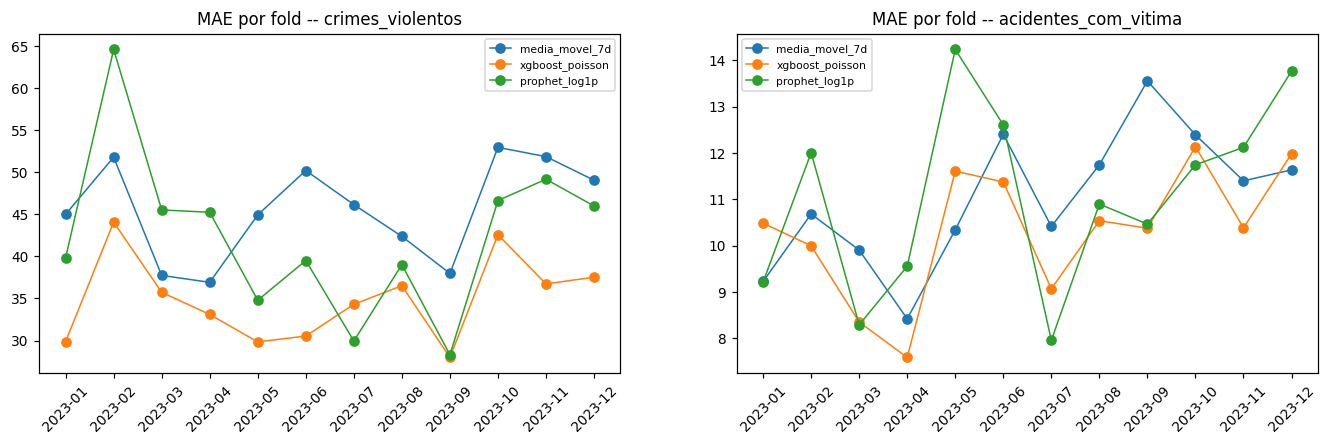
\includegraphics[width=.85\linewidth]{figuras/mae_por_fold.png}
\caption{MAE por \emph{fold} mensal, XGBoost Poisson vs.\ baselines e
Prophet}
\label{fig:mae-fold}
\end{figure}

Para a classificação de pico, uma Regressão Logística balanceada foi o
único classificador com Recall e PR-AUC úteis simultaneamente para
sinistros com vítima (Recall $=0,576$, $F_1=0,465$, PR-AUC $=0,476$;
Tabela~\ref{tab:classificacao}, Figura~\ref{fig:confusao}). Para crimes
violentos, nenhum modelo combina Recall e PR-AUC úteis: o \emph{Random
Forest} tem a melhor PR-AUC ($0,348$) mas Recall de apenas $0,05$ (26
falsos positivos foram necessários para acertar 1 verdadeiro no split
único da Etapa 14), e a heurística de dia da semana tem o melhor Recall
($0,50$) mas PR-AUC baixa ($0,115$). Por importância de atributos (medida
por \texttt{total\_gain}, não pelo \texttt{gain} médio isolado, que infla
atributos binários raros), 0 atributos de futebol aparecem no top 15 de
nenhum dos dois alvos.

\begin{table}[ht]
\centering
\caption{Desempenho de classificação de pico, \emph{pooled}
\emph{walk-forward}}
\label{tab:classificacao}
\small
\begin{tabular}{@{}llrrrrr@{}}
\toprule
\textbf{Alvo} & \textbf{Modelo} & \textbf{Acur.} & \textbf{Prec.} & \textbf{Recall} & \textbf{$F_1$} & \textbf{PR-AUC} \\
\midrule
Crimes violentos & Classe majoritária   & $0,945$ & $0,000$ & $0,000$ & $0,000$ & --      \\
Crimes violentos & \texttt{dia\_semana\_risco} & $0,515$ & $0,057$ & $0,500$ & $0,102$ & $0,115$ \\
Crimes violentos & Regressão Logística  & $0,680$ & $0,020$ & $0,100$ & $0,033$ & $0,228$ \\
Crimes violentos & XGBoost              & $0,917$ & $0,000$ & $0,000$ & $0,000$ & $0,201$ \\
Crimes violentos & Random Forest        & $0,942$ & $0,333$ & $0,050$ & $0,087$ & $0,348$ \\
\midrule
Sinistros c/ vítima & Classe majoritária  & $0,746$ & $0,000$ & $0,000$ & $0,000$ & --      \\
Sinistros c/ vítima & \texttt{dia\_semana\_risco} & $0,470$ & $0,228$ & $0,457$ & $0,304$ & $0,291$ \\
Sinistros c/ vítima & XGBoost             & $0,718$ & $0,308$ & $0,087$ & $0,136$ & $0,394$ \\
Sinistros c/ vítima & Random Forest       & $0,760$ & $0,647$ & $0,120$ & $0,202$ & $0,400$ \\
Sinistros c/ vítima & \textbf{Regressão Logística} & $0,663$ & $0,390$ & $\mathbf{0,576}$ & $\mathbf{0,465}$ & $\mathbf{0,476}$ \\
\bottomrule
\end{tabular}
\end{table}

\begin{figure}[ht]
\centering
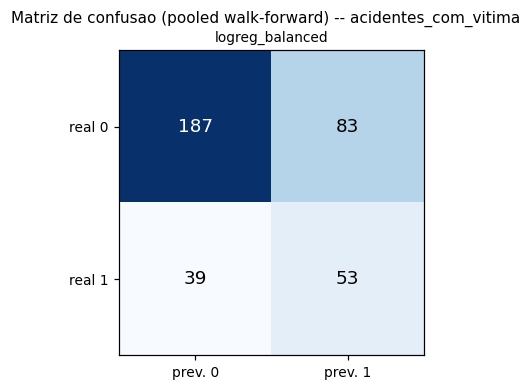
\includegraphics[width=.7\linewidth]{figuras/matriz_confusao_acidentes.png}
\caption{Matriz de confusão \emph{pooled}, Regressão Logística balanceada,
sinistros com vítima}
\label{fig:confusao}
\end{figure}

\subsection{Interpretabilidade (SHAP)}

Os valores de SHAP mostraram que histórico do próprio desfecho e
calendário/sazonalidade dominam a explicação da previsão nos três modelos
de produção (2 de regressão -- XGBoost Poisson -- e 1 de classificação --
Regressão Logística balanceada, treinados sobre todo o histórico com os
hiperparâmetros da Etapa 17); o grupo de atributos de futebol respondeu
por $2,2\%$ do total em crimes violentos, $18,7\%$ em sinistros com vítima
(regressão) e $26,6\%$ na classificação (Figura~\ref{fig:beeswarm}). Uma
auditoria específica revelou, porém, que esse peso bruto é
majoritariamente artefato: atributos como ``dias desde o último jogo''
têm SHAP elevado por serem proxies quase perfeitos de época do ano
(correlação de $-0,44$ com o mês; 80--96 dias em janeiro--março contra
$\sim$2 na temporada), mas correlação nula e não significativa com o alvo
já dessazonalizado ($\rho=-0,055$, $p=0,14$). Auditando as 18 variáveis de
futebol de cada modelo contra o alvo dessazonalizado, todas as 18 foram
marcadas como artefato nos três modelos -- a participação líquida do
futebol caiu para $0,0\%$ nos três (Figura~\ref{fig:futebol}), estável
também sob hiperparâmetros rasos (variação bruta de até 5,7 pontos
percentuais, líquida sempre $0,0\%$).

\begin{figure}[ht]
\centering
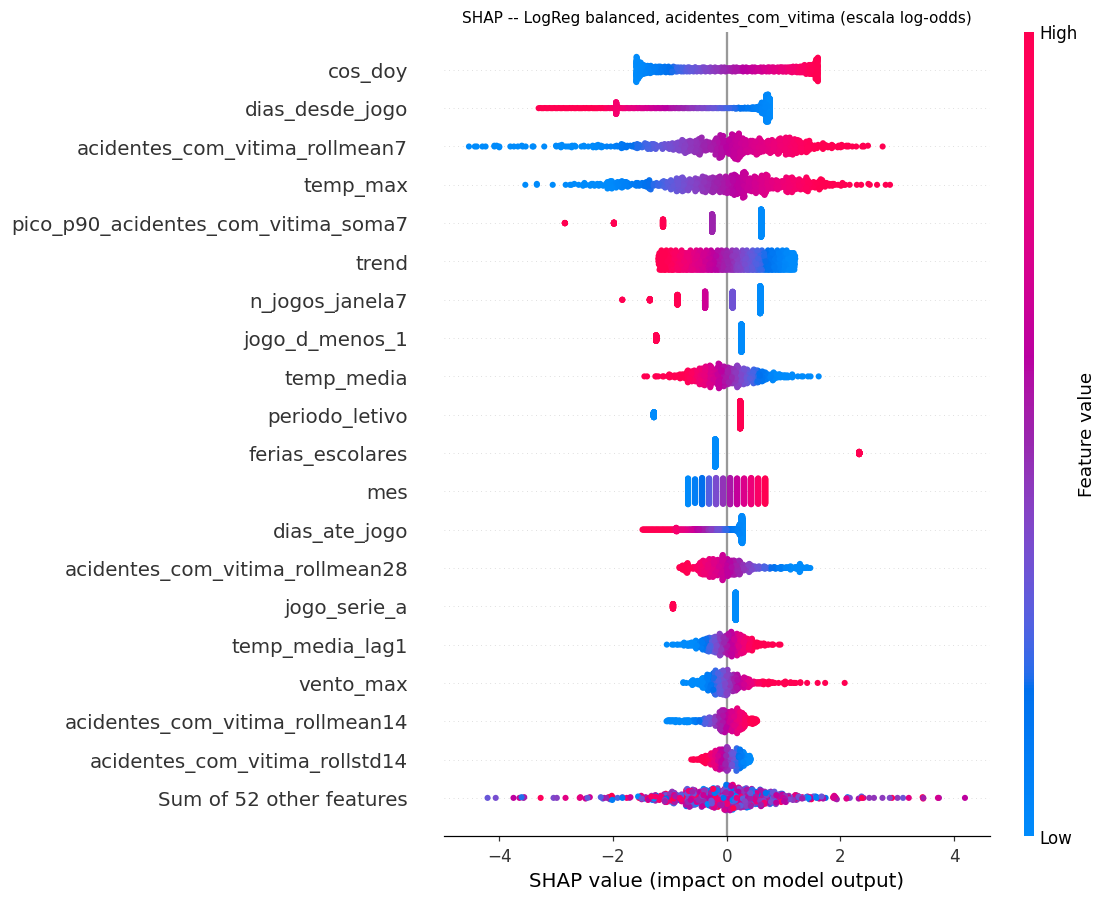
\includegraphics[width=.85\linewidth]{figuras/shap_beeswarm_acidentes.png}
\caption{\emph{Beeswarm} SHAP, XGBoost Poisson, sinistros com vítima}
\label{fig:beeswarm}
\end{figure}

\begin{figure}[ht]
\centering
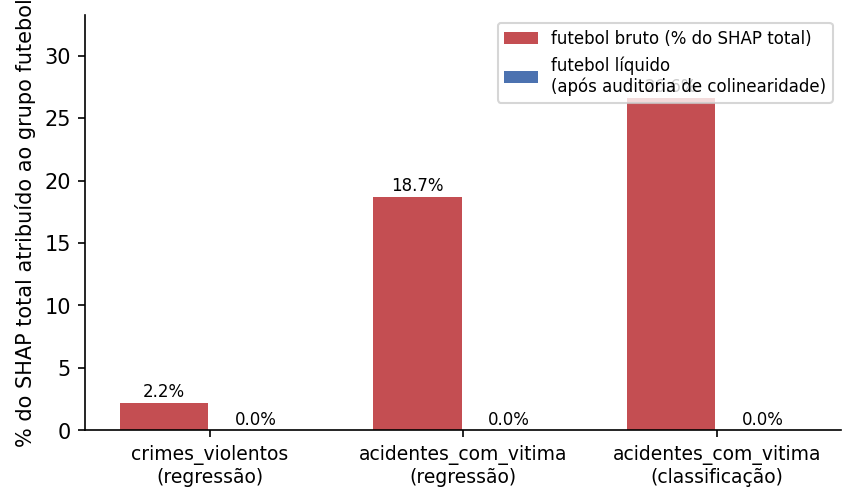
\includegraphics[width=.9\linewidth]{figuras/futebol_liquido.png}
\caption{Participação do grupo de atributos de futebol no SHAP total,
bruta e líquida de artefato de colinearidade com calendário, nos três
modelos de produção}
\label{fig:futebol}
\end{figure}

\subsection{Análise de cenários}

Simulações de cenário sobre dias reais (domingo com jogo comum, domingo
com clássico, quarta-feira com jogo noturno, domingo com clássico sob
chuva) estimaram, para sinistros com vítima, probabilidades de pico de
$0,855$, $0,539$, $0,627$ e $0,465$, contra $0,203$--$0,177$ em referências
sem jogo pareadas por dia da semana e época do ano. O cenário de maior
risco previsto foi o de jogo comum, não o clássico: a decomposição
aditiva do SHAP mostrou que a diferença é explicada por características
incidentais do dia-âncora (histórico recente, clima), não pelo tipo de
jogo -- ilustrando por que comparar cenários sem decompor a contribuição
de cada grupo de atributos pode induzir a uma leitura causal equivocada.

\section{Discussão}

O contraste com a literatura de referência
\cite{kurland2014,ristea2018,ristea2020} é informativo. Esses trabalhos,
em janelas espaciais de poucos quilômetros em torno de um único estádio,
encontraram associações mensuráveis entre dia de jogo e criminalidade
local; aqui, na escala da cidade e do dia inteiros, a associação bruta
observada desapareceu sistematicamente após controle por calendário, e
nenhum dos sete métodos independentes aplicados encontrou evidência
robusta em contrário. Isso não contradiz a literatura internacional: é
compatível com o problema da unidade de área modificável (MAUP), pelo qual
um efeito real e espacialmente concentrado pode se diluir ao ser agregado
à cidade inteira. O caso do Morumbi, cujo RR aparente de $2,39$ se revelou
artefato de três mecanismos concretos -- concentração em duas datas
extremas (final e semifinal da Copa do Brasil 2023), \emph{pile-up} de
geocodificação ($\sim$60\% dos registros nas coordenadas do próprio
estádio) e composição majoritariamente de furto simples ($75\%+$), não de
crime violento --, ilustra esse mecanismo dentro do próprio estudo -- não
uma prova de que o efeito local da literatura seja inexistente, mas
evidência de que a escala de análise importa tanto quanto o método
estatístico. Especificamente ao contexto
brasileiro, com três clubes de série A mandando jogos na capital e agenda
cobrindo quase todo o ano, ``dia de jogo'' em São Paulo é frequente (126
de 730 dias) e fortemente concentrado em fins de semana -- o próprio fator
de confusão identificado --, aproximando-se mais de uma característica
rotineira do calendário do que de um evento raro e saliente.

Do ponto de vista preditivo, o desempenho assimétrico entre os alvos --
sinistros com vítima admitiram um classificador de pico útil, crimes
violentos não -- é mais provavelmente explicado por diferenças na própria
dinâmica temporal de cada série (o histórico do desfecho domina o SHAP em
ambos) do que por qualquer variável de futebol. O fato de a otimização de
hiperparâmetros não ter produzido ganho relevante reforça essa leitura:
com 730 dias disponíveis, o fator limitante da previsão é a quantidade de
sinal nas variáveis explicativas, não a capacidade dos algoritmos.

Do ponto de vista prático, a implicação para o planejamento operacional
em São Paulo é direta: como o grupo de atributos de futebol não carrega
sinal líquido em nenhum dos três modelos, alocar efetivo policial ou de
fiscalização de trânsito com base no calendário de jogos, isoladamente,
não é uma estratégia sustentada pelos dados -- calendário civil (dia da
semana, mês, feriado) e o padrão histórico recente do próprio desfecho são
os insumos que de fato carregam sinal preditivo. O achado colateral do
teste de Fisher (Seção~4.1), que perderia significância estatística sob
qualquer um de três ajustes triviais (remoção do artefato de lote,
correção de Bonferroni, ou simplesmente notar que já é capturado pela
variável de fim de semana), ilustra por que decisões de política pública
não deveriam se apoiar em testes isolados sem essas checagens de
robustez.

\section{Conclusão}

Este trabalho respondeu, com evidência quantitativa, às perguntas que o
orientaram. Existe associação bruta fraca entre jogos e violência/
sinistros em alguns desfechos específicos, mas não sobrevive ao controle
por calendário em nenhuma das sete abordagens aplicadas -- sem evidência
de causalidade. Clássicos e jogos noturnos não apresentam risco maior que
jogos comuns e diurnos, descontado o artefato de colinearidade
identificado no SHAP; a influência do público não pôde ser testada, por
ausência dessa variável; e não há período de maior risco antes, durante
ou depois do jogo (nenhuma das 30 defasagens D$-2$ a D$+2$ foi
significativa após correção). As variáveis que de fato explicam os picos
são o histórico do próprio desfecho, o calendário e o clima -- o grupo de
futebol, auditado quanto à colinearidade, explica $0,0\%$ da previsão nos
três modelos avaliados.

O melhor modelo de regressão foi um XGBoost Poisson para os dois alvos; o
melhor classificador de pico foi uma Regressão Logística balanceada,
apenas para sinistros com vítima (Recall $0,576$--$0,674$) -- para crimes
violentos, nenhum classificador atingiu um ponto de operação útil. A
previsão com um dia de antecedência mostrou-se possível e validada fora
da amostra (\emph{walk-forward}), com margem de erro de $34,8$ crimes
violentos/dia (MAPE $7,1\%$) e $10,3$ sinistros com vítima/dia (MAPE
$12,7\%$); horizontes maiores que um dia não foram testados. Em suma, um
sistema de alerta de picos para São Paulo deve se apoiar no padrão
histórico do próprio desfecho, no calendário civil e no clima -- não no
calendário de jogos de futebol.

\section{Limitações}

Este estudo tem limitações de qualidade e cobertura de dados, variáveis
não observadas e desenho causal. A base de futebol cobre apenas
Campeonato Brasileiro (Séries A/B/C) e Copa do Brasil -- Paulistão e
Libertadores aparecem como ``sem jogo'', o que tende a atenuar qualquer
efeito real e inflar o peso do calendário. O público pagante é
integralmente ausente, impedindo testar se seu tamanho modula o risco. A
janela de sobreposição das três fontes é curta (730 dias), limitando a
validação temporal e a sazonalidade anual do Prophet. Cerca de 20\% das
coordenadas de crime são nulas, zero ou externas ao município -- por isso
o bairro, não a coordenada bruta, foi adotado como unidade primária da
análise espacial, com o anel de distância como robustez secundária. Há
lacunas e
censura de registro tratadas como ausência (não como zero), e um dia de
registro em lote tratado como dado ausente, com sensibilidade favorável à
conclusão qualitativa. A agenda de jogos não tem variação exógena
conhecida (decidida por federações e TV, não sorteada), o que impede
excluir por completo confundidores não observados -- mudanças de
policiamento ou eventos coincidentes não podem ser descartados com 730
dias de dados. Por fim, para crimes violentos nenhum classificador
atingiu um ponto de operação útil, e o horizonte de previsão avaliado foi
sempre de um dia.

\section{Trabalhos Futuros}

Cinco direções decorrem das limitações identificadas: (i) integrar uma
fonte de público pagante por partida, testando se a magnitude da
aglomeração modula o risco; (ii) incluir Campeonato Paulista e
Libertadores, reduzindo a atenuação identificada; (iii) estender o
horizonte de previsão para dois ou mais dias de antecedência; (iv) usar
modelos espaço-temporais que preservem a granularidade de bairro sem o
problema de geocodificação identificado aqui, no espírito dos trabalhos
de referência; e (v) buscar delineamentos com variação mais próxima da
exógena -- mudanças de mando de campo ou realocações de jogos por motivos
alheios ao calendário -- para identificação causal mais forte que a
disponível em dados observacionais.

\begin{thebibliography}{9}

\bibitem{cohen1979} Cohen, L.~E. and Felson, M. (1979) ``Social change and
crime rate trends: a routine activity approach''. \emph{American
Sociological Review}, 44(4), pp.~588--608.

\bibitem{kurland2014} Kurland, J., Johnson, S.~D. and Tilley, N. (2014)
``Offenses around stadiums: a natural experiment on crime attraction and
generation''. \emph{Journal of Research in Crime and Delinquency}, 51(1),
pp.~5--28.

\bibitem{ristea2018} Ristea, A., Kurland, J., Resch, B., Leitner, M. and
Langford, C. (2018) ``Estimating the spatial distribution of crime events
around a football stadium from georeferenced tweets''. \emph{ISPRS
International Journal of Geo-Information}, 7(2), 43.

\bibitem{ristea2020} Ristea, A., Al Boni, M., Resch, B., Gerber, M.~S. and
Leitner, M. (2020) ``Spatial crime distribution and prediction for sporting
events using social media''. \emph{International Journal of Geographical
Information Science}, 34(9), pp.~1708--1739.

\bibitem{austin2011} Austin, P.~C. (2011) ``An introduction to propensity
score methods for reducing the effects of confounding in observational
studies''. \emph{Multivariate Behavioral Research}, 46(3), pp.~399--424.

\bibitem{bh1995} Benjamini, Y. and Hochberg, Y. (1995) ``Controlling the
false discovery rate: a practical and powerful approach to multiple
testing''. \emph{Journal of the Royal Statistical Society, Series B},
57(1), pp.~289--300.

\bibitem{chen2016} Chen, T. and Guestrin, C. (2016) ``XGBoost: a scalable
tree boosting system''. In: \emph{Proceedings of the 22nd ACM SIGKDD
International Conference on Knowledge Discovery and Data Mining},
pp.~785--794.

\bibitem{taylor2018} Taylor, S.~J. and Letham, B. (2018) ``Forecasting at
scale''. \emph{The American Statistician}, 72(1), pp.~37--45.

\bibitem{lundberg2017} Lundberg, S.~M. and Lee, S.-I. (2017) ``A unified
approach to interpreting model predictions''. In: \emph{Advances in Neural
Information Processing Systems 30 (NeurIPS)}, pp.~4765--4774.

\bibitem{soliani2024} Soliani, R.~D., Argoud, A.~R.~T.~T., Santiago, F.,
Lopes, A.~V.~B. and Emekwuru, N. (2024) ``Catastrophic causes of truck
drivers' crashes on Brazilian highways: Mixed method analyses and crash
prediction using machine learning''. \emph{Multimodal Transportation},
3(4), 100173.

\bibitem{dasilva2025} da Silva, J.~P., Rodrigues-Jr, J.~F. and de
Albuquerque, J.~P. (2025) ``On the power of CNNs to detect slums in
Brazil''. \emph{Computers, Environment and Urban Systems}, 121, 102306.

\end{thebibliography}

\end{document}
